\section{Introducción}

Para este trabajo nos centraremos en resolver un problema real de aprendizaje automático utilizando el conocimiento obtenido a lo largo de las asignaturas de todo el Grado, con especial mención a los conocimientos adquiridos en las asignaturas \textit{Metaheurísticas} y \textit{Aprendizaje Automático}, y explorando nuevas técnicas de inteligencia artificial de cara a complementar dichos conocimientos de forma que se desarrolle un conocimiento en la exploración, formas de trabajo e investigación de nuevas técnicas.

\subsection{Problema a resolver}

De cara a la identificación de cadaveres, una de las tareas clave es la estimación de la edad. Aunque los forenses tenian formas de estimar a que edad murio una persona a partir de sus restos óseos, no existía un método concreto y universal de forma que el forense solo tuviera que seguir ciertas pautas y observar ciertas características de cara a la estimación de la edad.

Por este motivo, en el año 1920, Thomas Wingate Todd publicó un artículo científico \cite{todd} en el que proponía una forma de clasificar en diez rangos de edad los restos óseos de una persona fallecida a partir de ciertas características de la sínfisis púbica, de forma que el proceso de identificación de cadáveres fuera más sencillo para los forenses.

A pesar de ser una publicación de hace más de cien años, este método sigue siendo la base para la estimación de la edad a partir de los restos óseos. La mayoría de técnicas actuales se basan en esta propuesta y se siguen aplicando de forma manual.

El sistema propuesto por Todd se centraba en nueve características, asignándole distintos valores categóricos, de la sínfisis púbica para realizar su clasificación:

\begin{enumerate}
	\item Crestas y surcos: Porosidad regular, muy definidas, poco profundas, restos de surcos o no hay surcos.
	\item Superficie porosa irregular: No, medianamente o sí.
	\item Borde superior: Definido o no definido.
	\item Nódulo óseo: Ausente o presente.
	\item Borde inferior: Definido o no definido.
	\item Borde dorsal: Definido o no definido.
	\item Plataforma dorsal: Ausente o presente.
	\item Bisel ventral: Ausente, en proceso de formación o formado.
	\item Borde ventral: Ausente, parcialmente formado, formado sin excrecencias, formado con pocas excrecencias o formado con muchas excrecencias.
\end{enumerate}

\begin{table}[H]
\resizebox{\textwidth}{!}{%
	\begin{tabular}{|c|c|c|}
	\hline
	Crestas y surcos: Muy definidos & Superficie porosa irregular: Sí & Borde superior: Definido  \\ \hline
	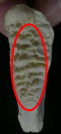
\includegraphics[scale = 0.75]{crestas_surcos_muy_definidos.png}  &   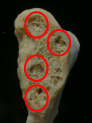
\includegraphics[scale = 0.75]{superficie_porosa_si.png} &  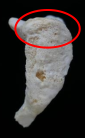
\includegraphics[scale = 0.75]{borde_superior_definido.png}  \\ \hline
	Nódulo óseo: Presente & Borde inferior: No definido & Borde dorsal: Definido \\ \hline
	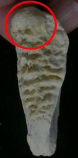
\includegraphics[scale = 0.75]{nodulo_oseo_presente.png} & 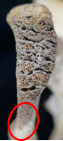
\includegraphics[scale = 0.75]{borde_inferior_no_definido.png} &  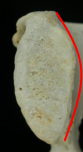
\includegraphics[scale = 0.75]{borde_dorsal_definido.png} \\ \hline
	Plataforma dorsal: Presente & Bisel ventral: En proceso de formación & Borde ventral: Muchas excrecencias \\ \hline
	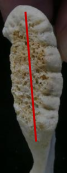
\includegraphics[scale = 0.75]{plataforma_dorsal_presente.png} & 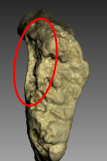
\includegraphics[scale = 0.75]{bisel_ventral_en_proceso_formacion.png} &   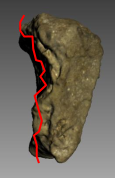
\includegraphics[scale = 0.75]{borde_ventral_muchas_excrecencias.png} \\ \hline
	\end{tabular}%
}
	\caption{Algunos ejemplos de las características consideradas por Todd.}\label{table:caracteristicas_todd}
\end{table}

En este trabajo propondremos una forma de automatizar este proceso de forma que sirva de ayuda al forense de cara a realizar su trabajo utilizando técnicas de inteligencia artificial y aprendizaje automático.

\subsubsection{Conjunto de datos}

Uno de los principales inconvenientes de este problema es que, como podemos ver, tenemos un gran número de características, de posibles valores para dichas características y de clases que asignar a cada dato, por lo que tendremos que buscar formas de reducir la dimensionalidad del problema.

Por otro lado, es muy dificil obtener un buen conjunto de datos para este problema. En nuestro caso utilizaremos un conjunto de datos clasificado manualmente por el Laboratorio de Antropología Física de la Universidad de Granada\cite{laboratorioForenseUGR}.

Este conjunto está formado por datos tomados de ambas lateralidades de la sínfisis púbica, siendo en total 892 datos distribuidos en los diez rangos de edades propuestos por Todd.

\begin{figure}[H]
	\centering
	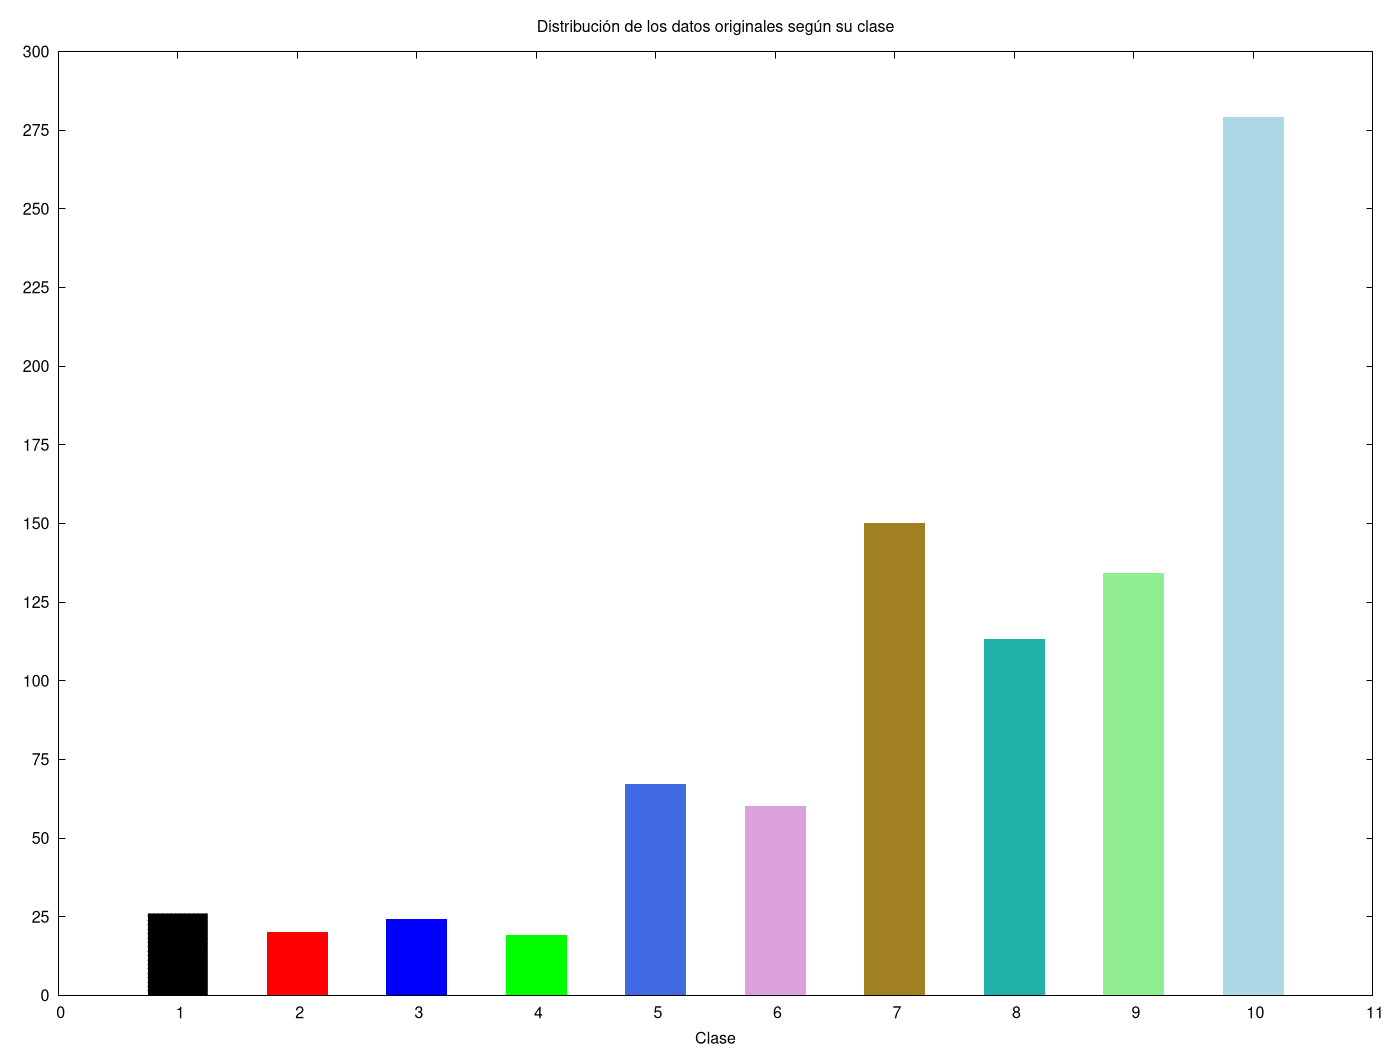
\includegraphics[scale = 0.30]{num_elementos_fase_original.png}
	\caption{Número de datos por cada clase con el conjunto de datos completo.}
	\label{fig:conteo_original}

\end{figure}

Como vemos, este conjunto de datos se encuentra claramente desbalanceado, hay muchas más muestras de las clases de edad más avanzada que de edades más bajas, además de contar con muy pocos en la mayoría de clases. Más adelante veremos como podemos solucionar estos problemas utilizando técnicas de sobremuestreo.

\subsection{Motivación}

Este trabajo está motivado ya que, aunque en los últimos años diversos modelos son capaces de obtener buenos resultados en esta clase de problemas, los modelos actuales apenas son interpretables por los expertos y esto no les permite utilizar estos modelos para avanzar en las técnicas de estimación de la edad a partir de restos óseos.

Por este motivo aparece la Inteligencia Artificial Explicable, y utilizando este tipo de técnicas intentaremos resolver el problema para que el experto sea capaz de entender y razonar como funciona el modelo.


\subsubsection{Inteligencia Artificial Explicable}

En la última década, gracias a los avances en la potencia computación, los distintos modelos de aprendizaje automático como las redes neuronales han revolucionado la inteligencia artificial. Estos nuevos modelos, a pesar de obtener resultados impensables con modelos clásicos, son demasiado complejos como para comprender la forma en la que funcionan internamente. Por este motivo ha aparecido el concepto de Inteligencia Artificial Explicable \cite{XAI} (XAI de sus siglas en inglés).

La inteligencia artificial explicable trata de expresar modelos de inteligencia artificial de una forma simple e interpretable. Con esto se busca que no solo los desarrolladores de dichos modelos sean capaces de comprobar y validar como funciona el modelo, sino que los usuarios sean capaces de entender a grandes rasgos como funciona, ya que en muchas ocasiones han de ser capaces de interpretar las decisiones del modelo para realizar su trabajo.

En este trabajo, debido a la complejidad del problema, así como que el experto que utilizará los resultados del modelo ha de ser capaz de interpretar, validar, y tomar decisiones con los resultados del modelo, se buscará obtener un modelo simple y fácilmente interpretable.


\subsection{Objetivos}

Tras introducir el problema, comentar los principales retos que nos podemos encontrar y orientar que tipo de solución buscamos, podemos distinguir estos claros objetivos:

\begin{enumerate}
	\item Reducir la dimensionalidad del problema.
	\item Equilibrar el número de datos de cada clase, así como obtener nuevos datos para las clases minoritarias.
	\item Estudiar, desarrollar y entrenar modelos que permitan una fácil interpretación.
\end{enumerate}


\newpage
